\documentclass[tikz]{standalone}
\usetikzlibrary{calc}
\usepackage{bm}
\usepackage{siunitx}
\begin{document}
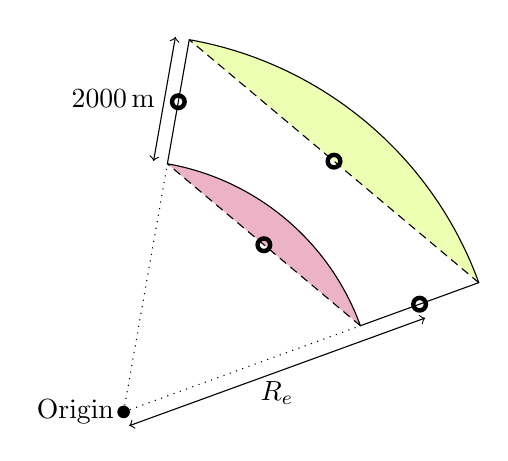
\begin{tikzpicture}[scale=0.8]
	\fill[white] (5,6) circle [radius=0.1];
	\fill (0,0) circle [radius=0.1] node [anchor=east] {Origin};
	\fill [purple!30] (20:4) arc (20:80:4);
	\fill [lime!30] (20:6) arc (20:80:6);
	\draw (20:4) arc (20:80:4) -- (80:6) arc (80:20:6) -- cycle;
	\draw [dotted] (0, 0) -- (80:4);
	\draw [dotted] (0, 0) -- (20:4);
	\draw [densely dashed] (20:4) -- (80:4);
	\draw [densely dashed] (20:6) -- (80:6);
	\draw [ultra thick] (20:5) circle [radius=0.1];
	\draw [ultra thick] (80:5) circle [radius=0.1];
	%\draw (50:6) circle [radius=0.1];
	%\draw (50:4) circle [radius=0.1];
	\draw [ultra thick] ($ (20:4) !.5! (80:4) $) circle [radius=0.1];
	\draw [ultra thick] ($ (20:6) !.5! (80:6) $) circle [radius=0.1];
	\draw [<->,transform canvas={yshift=-5,xshift=2}] (0,0) -- (20:5) node [midway,anchor=north] {$R_e$};
	\draw [<->,transform canvas={yshift=1,xshift=-5}] (80:4) -- (80:6) node [midway,anchor=east] {\SI{2000}{\meter}};
\end{tikzpicture}
\end{document}
